\documentclass[15pt]{sprawozdanie}
\usepackage{soul}

\class{Praca dyplomowa inżynierska}
\title{Opracowanie wirtualnego środowiska do symulacji dynamiki lotu bezzałogowych statków powietrznych}
\author{\textbf{inż. Wojciech Gajda} 304494\\\vspace{20pt}\textbf{Igor Faliszewski} 313223}
\instructor{dr inż. Paweł Kotowski}
\deadline{\today}

\graphicspath{{images/}}

\usepackage{amssymb}
\usepackage{amsmath}
\usepackage{polski}
\usepackage[utf8]{inputenc}
\usepackage{hyperref}
\usepackage{blindtext}
\usepackage{multicol}
\usepackage{multirow}
\usepackage{wrapfig}
\usepackage{float}
\usepackage{enumitem}
\usepackage{xfrac}
\usepackage{caption}
\usepackage{subcaption}
\usepackage{booktabs}
\usepackage{wasysym}
\usepackage{xcolor}
\usepackage{listings}
\usepackage{pdfpages}
\usepackage{fontspec}
\usepackage{comment}
\setmainfont{Verdana}
\usepackage[nochapter,owncaptions]{vhistory}
	
\usepackage{color, colortbl}
\definecolor{Gray}{gray}{0.9}

\definecolor{mGreen}{rgb}{0,0.6,0}
\definecolor{mGray}{rgb}{0.5,0.5,0.5}
\definecolor{mPurple}{rgb}{0.58,0,0.82}
\definecolor{backgroundColour}{rgb}{0.95,0.95,0.92}

\lstdefinestyle{CStyle}{
    backgroundcolor=\color{backgroundColour},   
    commentstyle=\color{mGreen},
    keywordstyle=\color{magenta},
    numberstyle=\tiny\color{mGray},
    stringstyle=\color{mPurple},
    basicstyle=\footnotesize,
    breakatwhitespace=false,         
    breaklines=true,                 
    captionpos=b,                    
    keepspaces=true,                 
    numbers=left,                    
    numbersep=5pt,                  
    showspaces=false,                
    showstringspaces=false,
    showtabs=false,                  
    tabsize=2,
    language=C
}

\usepackage[
backend=biber
,style=ieee
,sorting=none
]{biblatex}
\addbibresource{bibliografia.bib}
\DeclareNameAlias{author}{last-first}

\DeclareCiteCommand{\supercite}[\mkbibsuperscript]
  {\iffieldundef{prenote}
     {}
     {\BibliographyWarning{Ignoring prenote argument}}%
   \iffieldundef{postnote}
     {}
     {\BibliographyWarning{Ignoring postnote argument}}}
  {\usebibmacro{citeindex}%
   \bibopenbracket\usebibmacro{cite}\bibclosebracket}
  {\supercitedelim}
  {}
  
  \DeclareLabelalphaTemplate{
  \labelelement{
    \field[final]{shorthand}
    \field{label}
    \field[strwidth=3,strside=left,ifnames=1]{labelname}
    \field[strwidth=1,strside=left,final]{labelname}
    \field{labeltitle}
  }
  \labelelement{
    \field[strwidth=2,strside=right]{year}
  }
}

\let\cite=\supercite

\renewcommand*{\figurename}{Rys.}

\usepackage{titlesec}
\titlelabel{\thetitle.\quad}

\usepackage{tikz}


\usetikzlibrary{matrix, ,backgrounds}
\usepackage{array}

\makeatletter
\tikzset{SWOT/.style={matrix of nodes,inner sep=0pt,row sep=0pt,column sep=0pt,
cells={nodes={anchor=center,inner sep=2pt}},
column 1/.style={nodes={rotate=90,minimum height=8mm}},
ampersand replacement=\&,
execute at end matrix={\begin{scope}[on background layer]
 \fill[black!10] (\tikz@fig@name.west|-\tikz@fig@name-2-2.north) rectangle 
  (\tikz@fig@name-\the\pgfmatrixcurrentrow-2.south west);
\end{scope}
\draw (\tikz@fig@name.west|-\tikz@fig@name-2-2.north) rectangle 
(\tikz@fig@name-\the\pgfmatrixcurrentrow-\the\pgfmatrixcurrentcolumn.south east)
 (\tikz@fig@name-1-2.north west) rectangle 
(\tikz@fig@name-\the\pgfmatrixcurrentrow-\the\pgfmatrixcurrentcolumn.south east)
(\tikz@fig@name-2-2.center|-\tikz@fig@name.north) --
 (\tikz@fig@name-2-2.center|-\tikz@fig@name.south)
foreach \XX in {2,...,\the\numexpr\pgfmatrixcurrentrow-1}
{(\tikz@fig@name-\XX-2.south-|\tikz@fig@name.west) --
(\tikz@fig@name-\XX-2.south-|\tikz@fig@name.east) };
}}}
\makeatother

\usepackage{tocloft}
\renewcommand\cftfigfont{\small}

\renewcommand{\vhversionname}{Nr rewizji}
\renewcommand{\vhdatename}{Data}
\renewcommand{\vhauthorname}{Autor}
\renewcommand{\vhchangename}{Opis zmian}
\renewcommand\vhAuthorColWidth{.6\hsize} 
\renewcommand\vhChangeColWidth{1.4\hsize}

\setlength{\parindent}{0pt}

\begin{document}
%%\maketitle

\includepdf[pages=-]{first_page.pdf}


\section*{Streszczenie}
W pracy opisano realizację systemu przeznaczonego do symulacji dynamiki lotu bezzałogowych statków powietrznych. System pozwala na prowadzenie symulacji lotu w czasie rzeczywistem, który dodatkowo jest prezentowany jest w postaci trójwymiarowej wizualizacji. W trakcie wykonywania lotu logowane są dane i mogą zostać wykorzystane do analizy lotu. Opracowany został uniwersalny model dynamiki pozwalający na swobodną konfigurację parametrów statku. Obejmuje on modyfikację właściwości mechanicznych, aerodynamicznych oraz konfigurację zespołów napędowych i~wpływu czynników zewnętrznych. Symulacja dynamiki rozszerzona została o system sterowania. System został zaprojektowany w sposóbu ułatwiający zmianę parameterów statków i symulacji, tworzenie nowych konfiguracji statków oraz tworzenie i strojenie systemów sterowania. W pracy zaprezentowane zostało działanie systemu dla przykładowych modeli latających: stałopłatowca, wielowirnikowca i rakiety.

\section*{Słowa kluczowe}

symulacja, grafika komputerowa 3D, bezzałogowy statek powietrzny, model dynamiki ruchu

\newpage

\section*{Abstract}

\section*{Keywords}

\newpage
\tableofcontents

\newpage

\section{Historia zmian}
\begin{versionhistory}
  \vhEntry{0.0}{10.08.23}{Wojciech Gajda}{Utworzenie dokumentu, podstawowa struktura}
  \vhEntry{0.1}{11.10.23}{Wojciech Gajda}{Dostosowanie dokumentu do wymogów edytorskich, dodanie streszczenia}
  \vhEntry{0.2}{15.10.23}{Wojciech Gajda|Igor Faliszewski}{Dodanie  słownika, specyfikacji, analizy SWOT i bibliografii}
  \vhEntry{1.0}{16.10.23}{Wojciech Gajda|Igor Faliszewski}{Wydanie zgłoszone do L1}
\end{versionhistory}

\newpage

\section{Słownik pojęć}

\textbf{Statek powietrzny} -- urządzenie zdolne do unoszenia się (lotu) w atmosferze. Statek powietrzny jest zdolny w sposób aktywny wpływać na kierunek i prędkość lotu. W przeciwieństwie do formalnej definicji termin obejmuje również konstrukcję niewykorzystujące oddziaływania powietrza w locie (rakiety).\\

\textbf{Bezzałogowy statek powietrzny, BSP} -- statek powietrzny, który nie wymaga do lotu załogi obecnej na pokładzie oraz nie ma możliwości zabierania pasażerów, pilotowany zdalnie lub wykonujący lot autonomicznie.\\ 

\textbf{Pocisk} -- obiekt wystrzelony lub upuszczony ze statku powietrznego, nieposiadający własnego napędu. Porusza się na wskutek oddziaływania pola grawitacji i wpływu powietrza. Nie posiada wyróżnionej orientacji.\\

\textbf{Ładunek} -- pocisk, na ogół upuszczany, który pozostaje związany z statkiem powierzanym na sprężysto-tłumiącej linie. \\

\textbf{Stan obiektu} -- Opis położenia, orientacji i prędkości obiektu (pocisku lub statku powietrznego). Stan może zostać rozszerzony o dodatkowe informacje, takie jak: prędkości obrotowe poszczególnych silników, położenie powierzchni sterowych itd. \\

\textbf{Silnik fizyczny, silnik dynamiki} -- program komputerowy, którego zadaniem jest obliczenie położenia, orientacji i prędkości (kinematyki) statków powietrznych w zależności od sił działających na obiekt (dynamiki). \\

\textbf{Regulator} -- układ odpowiedzialny za generowanie rozkazów sterujących w oparciu o aktualny i zadany stan obiektu.\\

\textbf{Silnik graficzny} -- program komputerowy, którego zadaniem jest wizualizacja stanu obiektów i otoczenia.\\

\textbf{Agregator} --  program komputerowy, którego zadaniem jest zarządzaniem stanem aplikacji, obsługa przyłączających się aplikacji klienckich i zarządzanie procesami.\\


\newpage

\section{Wstęp}

\subsection{O projekcie}

Symulacje komputerowe dynamiki ruchu stanowią użyteczne narzędzie w pracach inżynierskich. Pozwalają na analizę poprawności działania układu mechanicznego przed jego wyprodukowaniem. W szczególności w zagadnieniu jakim jest projektowanie bezzałogowych statków powietrznych, zastosowanie symulacji pozwala zminimalizować koszty wytworzenia poprawnie działającego systemu.

\subsection{Przegląd istniejących rozwiązań}

Historia symulatorów lotu sięga lat 30 XX wieku. Pierwotnie zastosowanie symulatorów sprowadzało się do szkolenia pilotów cywilnych i wojskowych. W znanej obecnie formie kompletne symulatory lotu stanowią rozbudowane systemy integrujące wysokiej klasy oprogramowanie z peryferiami mającymi wierne odwzorowanie kokpitu kierowanej maszyny. Symulatory wykorzystywane do treningu pilotów podlegają rygorystycznym regulacją prawnym i na ogół ich zadaniem jest odwzorowanie jednej konkretnej maszyny. Równolegle uproszczone wersje symulatorów zaczeły zyskiwać popularność w zastosowaniu cywilnym, jako element rozrywki. W szczególności gry komputerowe związane z lotem bardzo często poświęcały zgodność z model rzeczywistym na rzecz lepszych odczuć użytkownika.\\

Na rynku dostępnych jest wiele środowisk symulacyjnych o różnym stopniu szczegółowości. Pełne systemy lotu stanowią produkt komercyjny projektowany na indywidualne zamówienie. Do najpopularniejszych dostępnych systemów sprzedawanych jako zamkniete oprogramowanie należą m. in.:

\begin{itemize}
\item Microsoft Flight Simulator -  seria komputerowych symulatorów lotu pozwalająca na symulację pilotowania różnych statków powietrznych. Założeniem jest wierne odtworzenie zachowania statków powietrznych, warunków pogodowych, jak również samych maszyn.
\item VBS (Arma) - środowisko symulacyjne do wizualizacji pola walki
\item Warthunder - darmowa gra komputerowa wprowadzająca znaczną ilość historycznych i współczesnych modeli samolotów, których parametry zostały oparte na dostępnych i odtajnych danych.
\item RealFlight - modelarski symulator lotu
\end{itemize}

Istnieją również rozwiązania typu open-source, realizujące jedynie poszczególne zadania:

\begin{itemize}
\item JSBsim - rozbudowany silnik dynamiki lotu działający w czasie rzeczywistym  
\item Ardupilot, INAV, Betaflight - kompletne systemy sterowania dla modeli zdalnie sterowanych
\end{itemize}


\section{Specyfikacja}


\subsection{Cel projektu}

Celem niniejszej pracy jest opracowanie wirtualnego środowiska do symulacji dynamiki lotu bezzałogowych statków powietrznych. System implementuje podstawowy model dynamiki statków powietrznych wyposażonych w silniki rotorowe, silniki odrzutowe, powierzchnie nośne i powierzchnie sterowe. Pozwala na przeprowadzenie lotu symulowanym obiektem którego parametry określane są przez konfigurację podaną przez użytkownika. System dzieli się na serwer i aplikacje kliencką. Różnorodność modułów pozwala na realizacje różnych scenariuszy min. strzał, upuszczenie ładunku, kolizje, wpływ warunków środowiskowych. Oprogramowanie jest w głównej mierze przeznaczone dla producentów bezzałogowych statków powietrznych, w celu umożliwienia przetestowania oraz dobrania odpowiednich parametrów BSP przed rzeczywistymi lotami próbnymi, co pozwoli na zminimalizowanie kosztów produkcji. Potencjalnymi klientami są również uczelnie z zamiarem wykorzystania oprogramowania w celach dydaktycznych oraz pasjonaci BSP.

\newpage
\subsection{Wymagania funkcjonalne}

W tabeli (\ref{use_case}) przedstawiono scenariusze wykorzystania oprogramowania.

\renewcommand{\arraystretch}{1.5}
\begin{table}[!h]
	\centering
	\begin{tabular}{|m{0.07\textwidth}|m{0.18\textwidth}|m{0.7\textwidth}|} 
		\hline
		\rowcolor{Gray}
		Aktor & Nazwa & Opis \\
		\hline
		\centering \multirow{4}{*}{\rotatebox[origin=c]{90}{Użytkownik}} 
		& Symulacja BSP & Możliwość zasymulowania lotu BSP.  \\
		\cline{2-3}
		& Różnorodne typy BSP & Możliwość zasymulowania BSP wyposażonych w silniki rotorowe, silniki odrzutowe, powierzchnie nośne i powierzchnie sterowe.  \\
		\cline{2-3}
		& Rój BSP & Możliwość zasymulowania wielu BSP jednocześnie. \\
		\cline{2-3}
		& Modele BSP i środowiska & Możliwość dodawania własnych modeli BSP oraz modeli map.\\
		\cline{2-3}
		& Konfiguracja & Możliwość konfigurowania parametrów serwera, wizualizacji i kontrolerów.\\
		\cline{2-3}
		& Interfejs użytkownika & Podczas symulacji użytkownik ma dostęp do informacji niezbędnych do lotu, a więc min. mapa, sztuczny horyzont, silniki. \\
		\cline{2-3}
		& Zdalna aplikacja kliencka & Możliwość zdalnego połączenia wizualizacji z serwerem wykorzystując protokół TCP/IP. \\
		\hline
		\centering \multirow{2.5}{*}{\rotatebox[origin=c]{90}{Analityk}} 
		& Testowanie parametrów BSP & Możliwość przetestowania własnych parametrów BSP w locie symulowanym i ich poprawianie. \\
		\cline{2-3}
		 & Analiza logów & Możliwość przeanalizowania lotu za pomocą logów utworzonych w czasie symulacji. \\ 
		 \cline{2-3}
		 & Symulacja warunków środowiskowych & Testowanie parametrów BSP w różnych warunkach środowiskowych (np. wiatr).\\ 
		\hline
		\centering \multirow{3}{*}{\rotatebox[origin=c]{90}{Deweloper}} 
		& Systemy\newline sterowania & Dodawanie i zarządzanie systemami sterowania. \\
		\cline{2-3}
		& Doskonalenie symulacji & Doskonalenie symulacji wykorzystując porównania logów symulacji z wynikami prawdziwych lotów próbnych.\\ 
		\hline
	\end{tabular}
	\caption{Scenariusze użycia -- use cases}
	\label{use_case}
\end{table}


\newpage
\subsection{Wymaganie niefunkcjonalne}

W tabeli (\ref{non_func}) przedstawiono wymagania niefunkcjonalne, które musi spełniać oprogramowanie.

\renewcommand{\arraystretch}{1.5}
\begin{table}[!h]
	\centering
	\begin{tabular}{|m{0.03\textwidth}|m{0.21\textwidth}|m{0.025\textwidth}|m{0.68\textwidth}|} 
		\hline
		\rowcolor{Gray}		\multicolumn{2}{c}{Wymagania} & No. & Opis \\
		\hline
		\centering \multirow{3}{*}{\rotatebox[origin=c]{90}{Usability}}
		&\multirow{1}{*}{Używalność} 
		& 1 & Użytkownik jest w stanie dopasować rozmiar okna wizualizacji i interfejsu do swoich potrzeb i ograniczeń sprzętu. \\
		\cline{3-4}
		& & 2 & Serwer da się uruchomić natywnie na Unixie lub w wirtualnym kontenerze Docker, a wizualizacja działa na wirtualnej maszynie Javy. \\
		\cline{3-4}
		& & 3 & Komunikacja między serwerem, a wizualizacją powinna pozwalać na responsywne sterowanie BSP. \\
		\cline{2-4}
		& \multirow{1}{*}{Ergonomia} 
		& 4 & Interfejs użytkownika powinien być przejrzysty i korzystać ze standardowych liczników wykorzystywanych w~lotnictwie.  \\
		\cline{3-4}
		& & 5 & Konfiguracja kontrolera powinna odbyć się bez znajomości użytkownika z interpretacją wejścia przez system.  \\
		\hline
		\centering \multirow{3}{*}{\rotatebox[origin=c]{90}{Reliability}}
		& \multirow{1}{*}{Dokładność} 
		& 6 & Dokładność symulacji powinna zależeć wyłącznie od błędów obliczeń i dokładności wprowadzonych parametrów. \\
		\cline{2-4}
		& \multirow{1}{*}{Sprawdzalność} 
		& 7 & Zgodność symulacji z rzeczywistością da się sprawdzić poprzez analizę logów oraz przez subiektywną opinię analityka. \\
		\hline
		\centering \multirow{1}{*}{\rotatebox[origin=c]{90}{Perf.}}
		& \multirow{1}{*}{Przepustowość} 
		& 8 & Wydajność serwera powinna skalować się względem liczby aktualnie symulowanych BSP. \\
		\hline
		\centering \multirow{3}{*}{\rotatebox[origin=c]{90}{Supportability}}
		& \multirow{1}{*}{Konserwacja} 
		& 9 &Systemy sterowania, elementy interfejsu i moduły konfigurowalne powinny być tak zaprojektowanie aby dodawanie nowych oraz modyfikacja istniejących była prosta i szybka.  \\
		\cline{3-4}
		& & 10 & System powinien być podzielony na moduły, które można niezależnie modyfikować. \\
		\cline{2-4}
		& \multirow{1}{*}{Audytowalność} 
		& 11 & W czasie lotu serwer powinien zapisywać logi z symulacji. \\
		\cline{2-4}
		& \multirow{1}{*}{Instalowalność} 
		& 12 & Proces instalacji serwera powinien być dobrze opisany i~prosty. Niewymagany w przypadku wizualizacji. \\
		\cline{2-4}
		& \multirow{1}{*}{Konfigurowalność} 
		& 13 & Oprogramowanie powinno umożliwiać konfigurację serwera, wizualizacji, modeli, kontrolerów, parametrów BSP. \\
		\hline
	\end{tabular}
	\caption{Wymaganie niefunkcjonalne - FURPS}
	\label{non_func}
\end{table}

\subsection{Architektura}
System został podzielony na moduły. Moduły komunikują się między sobą poprzez kolejki ZeroMQ. Jako warstwa transportowa wykorzystane są mechanizmy komunikacji wewnątrzprocesowej, międzyprocesowej i protokół TCP/IP. Moduły odpowiadają obiektom z domeny systemu.\\

\textbf{UAV\_physic\_engine} -- moduł odpowiedzialny symulację dynamiki statku powietrznego, uwzględniając wszystkie jego własciwości mechaniczne i wpływ otoczenia. Oblicza stan pojedynczego BSP w czasie rzeczywistym. \\

\textbf{UAV\_controller} -- moduł reprezentujący system sterowania statkiem powietrznym. Interpretuje stan statków powietrznych i buduje symulacje otoczenie. Symuluje działanie czujników pomiarowych, systemu filtracji, algorytmów nawigacji pokładowej oraz systemów sterowania i stabilizacji. Bezpośrednio wpływa na zachowanie symulacji dynamiki.\\

\textbf{UAV\_drop\_physic} -- moduł odpowiedzialny za obliczenie dynamiki pocisków. Oblicza stan wszystkich pocisków aktywnych w symulacji.\\

\textbf{UAV\_aggregator} -- moduł agregujący moduły symulacyjne z wizualizacją. Zarządza pracą pozostałych modeli i wprowadza niektóre zagadnienia otoczenia takie jak atmosferę, połączenia miedzy BSP, a ładunkami oraz kolizje.\\

\textbf{UAV\_server} -- definicja wirtualnego kontenera, odpowiedzialna zabudowanie wszystkich modułów składających się na serwer, tj. wszystkie z wyłączeniem wizualizacji. Ze zbudowanych modułów budowany jest obraz kontenera. Umożliwia to uruchomienie serwera na dowolnej maszynie wspierającej daną konteneryzację.\\

\textbf{UAV\_visualization} -- moduł odpowiedzialny za wyświetlenie  interfejsu użytkownika oraz obecnego stanu symulacji. Przekazuje dane wejściowe z kontrolera do systemu. Stanowi interfejs komunikacji użytkownika z systemem. \\

\newpage

\subsection{Dobór technologii}

Do realizacji poszczególnych modułów wybrane zostały następujące narzędzia programistyczne i biblioteki zewnętrzne.\\


\textbf{UAV\_physic\_engine, UAV\_controller i UAV\_drop\_physic}\\

Ze względu na duży nakład obliczeniowy -- symulacja w czasie rzeczywistym z krokiem całkowania rzędu 1ms -- wybrany został język C++. Z uwagi na swoją wydajność i elastyczność stanowi on naturalny wybór w wydajnych symulacjach komputerowych. Dodatkowo wykorzystane zostały następujące biblioteki:
\begin{itemize}[noitemsep,nolistsep]
	\item Eigen -- biblioteka zawierająca elementy algebry liniowej: macierze, wektory i związane z nimi algorytmy. Eigen stawia na wydajność poprzez wykorzystanie rozkadów typu SIMD, przy 		jednoczesnym zachowaniu przejrzystej składni,
	\item ZeroMQ -- binding biblioteki libzmq dla języka C++. Libzmq jest bazową biblioteką implementującą kolejki ZeroMQ,
	\item RapidXML -- biblioteka do parsowania plików XML,
	\item Cxxopts -- biblitoteka do interpretowania argumentów wejściowych programu.
\end{itemize}
\  \\
\textbf{UAV\_aggregator}\\

Do realizacji modułu agregatora wykorzystany zostanie język Rust. Pozwala on na tworzenie wydajnego i kompilowanego kodu przy jednoczesnym zachowaniu przenośności między systemami. Natywnie wspiera zarządzanie innymi procesami i udostępnia wiele bibliotek. Wykorzystane zostały następujące biblioteki:
\begin{itemize}[noitemsep,nolistsep]
	\item nalgebra -- biblioteka zawierająca do elementy algebry liniowej, odpowiednik biblioteki Eigen dla języka Rust,
	\item zmq -- binding biblioteki libzmq dla języka Rust. Libzmq jest bazową biblioteką implementującą kolejki ZeroMQ,
	\item xmltree -- biblioteka do parsowania plików XML,
	\item merkletree -- biblioteka wykorzystana do hashowania drzewa plików,
	\item sha1 -- biblioteka wykorzystana do hashowania plików konfiguracyjnych,
	\item serde\_yaml  - biblioteka do parsowania plików YAML.
\end{itemize}
\  \\
\textbf{UAV\_server}\\

Do realizacja kontenera wybrane zostało oprogramowanie Docker. Obraz został zdefiniowany przy pomocy Dockerfile i skryptów Bash. Przygotowany został również plik Docker compose ułatwiający uruchomienie serwera.

\newpage

\textbf{UAV\_visualization} -- JAVA. \\ 

Każdy z modułów znajduje się w oddzielnym repozytorium Git na platformie Github. Dla ułatwienia pracy z wykorzystaniem Github Actions przygotowane zostały odpowiednie mechanizmy CI/CD.


\newpage
\section{Harmonogram projektu}

Prace nad projektem zostały rozpoczęte 13.03.2023. Początkowe wersje modułów były rozwijane w lokalnych repozytoriach autorów. W czerwcu 2023 rozpoczęto integrację modułu, a zagadnienia zostały opisane w programie Jira. Rysunek (\ref{zamkniete_jira}) prezentuje zagadnienia zamknięte do 15.10.2023.

\begin{figure}[!h]
\centering
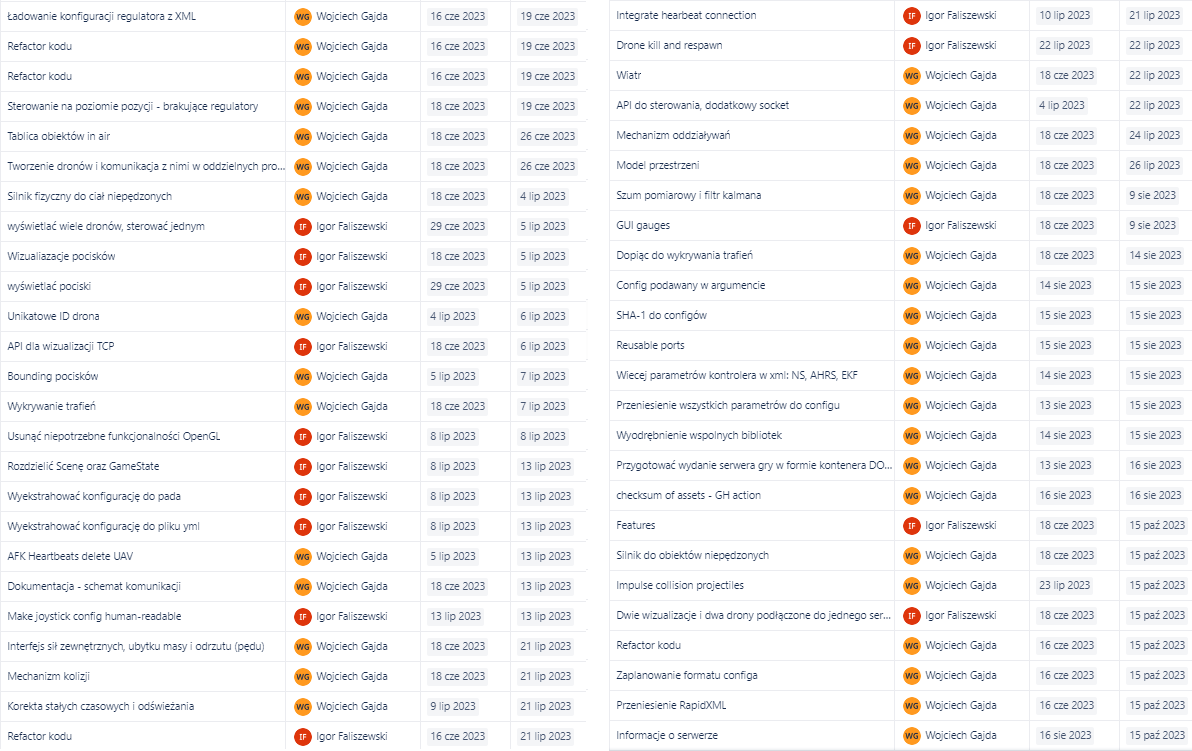
\includegraphics[width=\textwidth]{jira_june_sept.png}
\caption{Zgłoszenia zamknięte do 15.10.2023}
\label{zamkniete_jira}
\end{figure}

Na podstawie otwartych zagadnień i analizy założonej specyfikacji zaplanowany został harmonogram pracy zawierający zagadnienia których realizacja jest niezbędna do ukończenia projektu. Tabela (\ref{harmonogram}) prezentuje ww. harmonogram. 

\renewcommand{\arraystretch}{1.5}
\begin{table}
\centering
\begin{tabular}{|m{0.4\textwidth}|m{0.15\textwidth}|m{0.15\textwidth}|m{0.2\textwidth}|} 
\hline
\rowcolor{Gray}
Opis zadania & Data\newline rozpoczęcia & Data\newline zakończenia & Osoba\newline odpowiedzialna \\
 \hline
Dodanie różnych modeli pocisków i ładunków & 16.10.2023 & 23.10.2023 & Igor Faliszewski \\
 \hline
Dodanie nowych konfiguracji rakiet & 16.10.2023 & 29.10.2023 & Wojciech Gajda \\
 \hline
Generator konfiguracji kontrolera & 24.10.2023 & 29.10.2023 & Igor Faliszewski \\ 
\hline
Implementacja nowych regulatorów płatowców & 30.10.2023 & 19.11.2023 & Wojciech Gajda \\ 
\hline
Krzywa łańcuchowa & 30.10.2023 & 12.11.2023 & Igor Faliszewski \\ 
\hline
Określanie orientacji pocisków i~ładunków & 13.11.2023 & 19.11.2023 & Igor Faliszewski \\ 
\hline
GUI wyboru pocisku i ładunku & 20.11.2023 & 26.11.2023 & Igor Faliszewski \\ 
\hline
Rozwój klasy regulatorów PID & 20.11.2023 & 10.12.2023 & Wojciech Gajda \\ 
\hline
Radio & 27.11.2023 & 03.12.2023 & Igor Faliszewski \\ 
\hline
Generowanie assetów na podst. map terenu & 04.12.2023 & 31.12.2023 & Igor Faliszewski \\ 
\hline
Nazwy użytkowników nad statkami & 04.12.2023 & 10.12.2023 & Igor Faliszewski \\
 \hline
Dodatkowe algorytmy całkowania & 11.12.2023 & 31.12.2023 & Wojciech Gajda \\
 \hline
Dźwiek gry & 11.12.2023 & 18.12.2023 & Igor Faliszewski \\
 \hline
Limit FPS & 19.12.2023 & 23.12.2023 & Igor Faliszewski \\
 \hline
Zachowanie kamery w pobliżu ściany & 26.12.2023 & 31.12.2023 & Igor Faliszewski \\ 
\hline
Dokumentacja kodu & 16.10.2023 & 31.12.2023 & Wszyscy \\ 
\hline
Testy & 13.11.2023 & 31.12.2023 & Wszyscy \\
 \hline
Rozbudowa assetów & 30.10.2023 & 31.12.2023 & Wszyscy \\ 
\hline
\end{tabular}
\caption{Harmonogram projektu październik -- grudzień 2023}
\label{harmonogram}
\end{table}

\newpage
\section{Ocena ryzyka -- analiza SWOT}

\begin{table}[!h]
\begin{tikzpicture}
\renewcommand{\arraystretch}{1.2}
\setlist{left=1em,parsep=0.5ex,after=\smallskip}
\def\myw{7.5cm}
\matrix[SWOT] 
{
\& |[fill=black!10]|\renewcommand{\arraystretch}{1.3}\begin{tabular}{Wc{\myw}Wc{\myw}}
Pozytywne & Negatywne\\ 
\end{tabular}\\
 Wewnętrzne
  \& \begin{tabular}{p{\myw}p{\myw}}
	\textbf{Silne strony:} \begin{itemize}
 	 \item przejrzysta implementacja zgodna z paradygmatami programowania obiektowego,
        	 \item modułowość projektu, pozwalająca na modyfikację poszczególnych komponentów bez konieczności przebudowy całego projektu,
        	 \item uniwersalny model dynamiki statków powietrznych, pozwalający na obliczenia w czasie rzeczywistym.
\end{itemize}
& 
 \textbf{Słabe strony:} \begin{itemize}
  	\item ograniczony czas projektu może skutkować niedopracowaniami we wdrożonych funkcjonalnościach,
        \item obliczenia symulacji i kolizji obywają się na CPU, co może ograniczać wydajność,
        \item model matematyczny jest mniej dokładny niż rozbudowana symulacja mechaniki płynów.
\end{itemize} \end{tabular}\\
 Zewnętrzne \& \begin{tabular}{p{\myw}p{\myw}}
	\textbf{Szanse:} \begin{itemize}
   	\item dzięki udostępnieniu systemu na otwartej licencji, możliwe jest wykorzystanie wypracowanych rozwiązań w przyszłych projektach,
       	\item system może stanowić narzędzie ułatwiające opracowanie i testowanie nowatorskich systemów sterowania,
       	\item system może stanowić bezpłatną alternatywę dla komercyjnych symulatorów lotu.
\end{itemize} & \textbf{Zagrożenia:} \begin{itemize}
  \item język Rust wykorzystany w UAV\_aggregator może przestać być wspierany na przestrzeni najbliższych lat,
  \item trudności z identyfikacja wiarygodnych współczynników modelu dynamiki,
  \item rozbudowany system może okazać się trudny w obsłudze dla użytkownika.
  
\end{itemize} \end{tabular}\\
};
\end{tikzpicture}
\caption{Analiza SWOT}
\label{swot}
\end{table}





\newpage
\section{Bibliografia}

%\printbibliography
\nocite{*}

\printbibliography[type=book,heading=subbibliography,title={Literatura}]
\printbibliography[type=article,heading=subbibliography,title={Artykuły}]
\printbibliography[type=online,heading=subbibliography,title={Źródła internetowe}]

\end{document}\grid


\begin{comment}

Symulacje komputerowe dynamiki ruchu  W szczególności w zagadnieniu jakim jest projektowanie systemów sterowania do bezzałogowych statków powietrznych, zastosowanie takich narzędzi pozwala zminimalizować koszty wytworzenia poprawnie działającego systemu i przyśpieszyć jego rozwój i testowanie.

Celem niniejszej pracy jest opracowanie wirtualnego środowiska do symulacji dynamiki lotu bezzałogowych statków powietrznych. System implementuje podstawowy model dynamiki statków powietrznych wyposażonych w silniki rotorowe, silniki odrzutowe, powierzchnie nośne i powierzchnie sterowe. Pozwala na przeprowadzenie lotu symulowanym obiektem ktorego parametery określane są przez konfiguracje. System dzieli sie na serwer i aplikacje kliencką. Róznorodność modułów pozwala na realizacje róznych scenariusz (strzał, upuszczenie ładunku, kolizje, wpływ warunków srodowiskowych etc.)


\section{Model dynamiki statku powietrznego}

\begin{equation}
\begin{cases}
\dot{Y} =  T(Y) \cdot X + stabilizacja\\ 
A \cdot \dot{X} + \Omega (X) \cdot A \cdot X = F_g + F_a + F_d + F_o
\end{cases}
\end{equation}

gdzie:
\begin{itemize}
\item $Y$ - wektor pozycji i orientacji wyrażony w układzie globalnym
\item $X$ - wektor prędkości postępowej i kątowej w układzie związanym ze statkiem powietrznym
\item $A$ - macierz masowa
\item $\Omega$ - macierz gyroskopowa
\item $F_g$ - siła i moment pochodząca od siły grawitacji wyrażone w układzie związanym ze statkiem powietrznym
\item $F_a$ - siła i moment aerodynamiczny wyrażone w układzie związanym ze statkiem powietrznym
\item $F_d$ - siła i moment zespołów napędowych wyrażone w układzie związanym ze statkiem powietrznym
\item $F_o$ - siła i moment oddziaływań zewnętrznych napędowych wyrażone w układzie związanym ze statkiem powietrznym
\end{itemize}

\begin{equation}
Y = \begin{bmatrix}
x_{NED}\\
y_{NED}\\
z_{NED}\\
q_0\\
q_x\\
q_y\\
q_z
\end{bmatrix}
\end{equation}

\begin{equation}
X = \begin{bmatrix}
\dot{x}_b\\
\dot{y}_b\\
\dot{z}_b\\
P_b\\
Q_b\\
R_b
\end{bmatrix}
\end{equation}

\begin{equation}
F_g = R_{nb}(Y) \cdot  \begin{bmatrix}
0\\
0\\
g
\end{bmatrix}
\end{equation}

\begin{equation}
F_a = \frac{1}{2}\rho \cdot V_{tot}^2 S R_{wb} C_F \\
M_a = \frac{1}{2}\rho \cdot V_{tot}^2 S d R_{wb} C_F
\end{equation}

\end{comment}
